\documentclass{article}
\usepackage[utf8]{inputenc}
\usepackage[letterpaper]{geometry}
\usepackage{graphicx}
\graphicspath{ {./img} }

\title{PHYS 2411 Homework 1}
\author{Duncan Wilkie}
\date{10 September 2021}

\begin{document}

\maketitle

\section*{Problem 1}
The analytical formula for the Doppler effect is $f_o = f_s(1+v_{rel}/c)\Leftrightarrow v_{rel}=c(f_o/f_s-1)$.
Evaluating this at the values given in the problem yields $v_{rel}=(3\times 10^8)\left(\frac{103.3\times 10^6 + 9.44}{103.3\times10^6} - 1\right) = 27.415295256$. The program in the attatched script file computes this in two ways. 
The first algorithm results in $v_{rel}=20.788805008$ while the second results in $v_{rel}=27.4152946472168$.
Comparing this to the analytic solution found via the above method, the second clearly has much higher precision, since it agrees with the analytic solution to 5 digits.

\section*{Problem 2}
Refactoring the above program to use double instead of single precision, we get agreement to 13 digits of both algorithms with the analytical solution.

\section*{Problem 3}
The plot of the output data appears below.
\[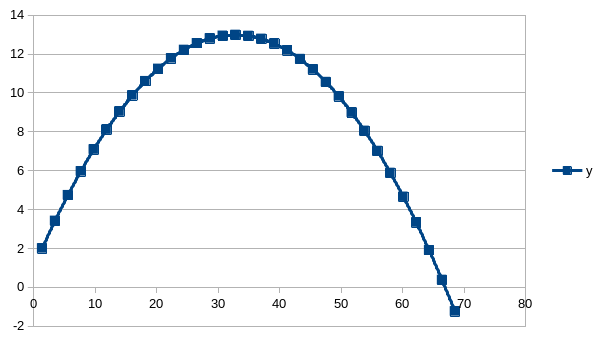
\includegraphics[scale=0.5]{plot3.png}\]
From the output data, the ball appears to hit the ground after about 3.1 seconds. 
\section*{Problem 4}\
The plot for $m=20$ is \[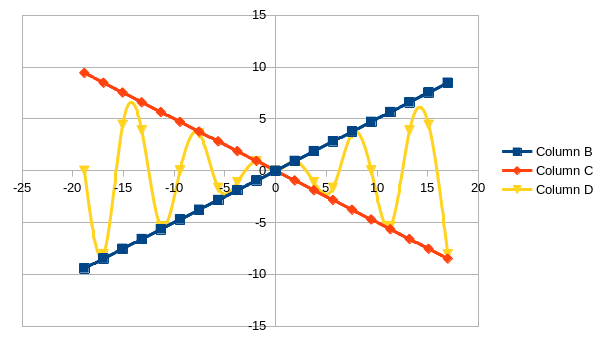
\includegraphics[scale=0.5]{plot1.png}\]
For $m=40$, we have \[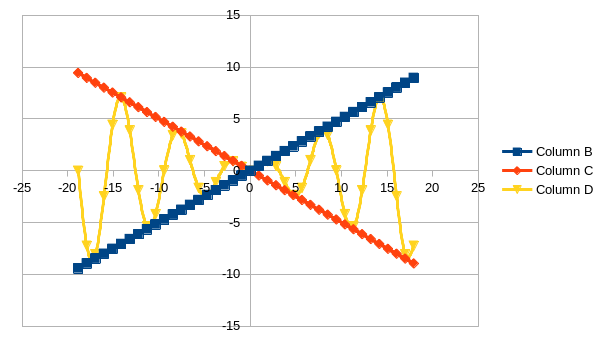
\includegraphics[scale=0.5]{plot2.png}\]

Evidently, the greater resolution makes the plots more accurate.
In the first plot, the curve misses the bounding line by a noticeable margin at its highest point, whereas in the second it touches it.
It is, of course, expected that it will touch the bounding line.

\section*{Script Files}
\subsection{}
\begin{verbatim}
Script started on Fri 10 Sep 2021 03:46:59 PM CDT
tput: unknown terminal "st-256color"
tcsh: No entry for terminal type "st-256color"
tcsh: using dumb terminal settings.
[dwilk14@tigers ~/HW1]$ cat p1.cpp
#include <iostream>
#include <iomanip>
using namespace std;

int main (){
  const float c=3.e8;  // speed of light, m/s
  float fs,fo,deltaf,vrel;  // fs, source frequency, Hz        
// fo, frequency detected by object, Hz
       // deltaf, frequency shift, Hz
       // vrel, object velocity, m/s
  fs=103.3e6;
  deltaf=9.44;

  cout << "Algorithm (i):" << endl;
  fo=fs+deltaf;
  vrel=fo*c-fs*c;
  vrel=vrel/fs;
  cout << "v=" << setprecision (15) << vrel << " m/s" << endl;

  cout << "Algorithm (ii):" << endl;
  vrel=deltaf*c/fs;
  cout << "v=" << setprecision (15) << vrel << " m/s" << endl;

  cout << "Just a check:" << endl;
  cout << "v=" << setprecision (15)
     << 9.44*(3.e8)/( (double) fs) << " m/s" << endl;

  return 0;
}
[dwilk14@tigers ~/HW1]$ g++ p1.cpp -o p1
[dwilk14@tigers ~/HW1]$ ./p1
Algorithm (i):
v=20.7888050079346 m/s
Algorithm (ii):
v=27.4152946472168 m/s
Just a check:
v=27.4152952565344 m/s
[dwilk14@tigers ~/HW1]$ cp dwilk14_hw1p1.txt /home3/kristina/phys2411/.
[dwilk14@tigers ~/HW1]$ exit
exit

Script done on Fri 10 Sep 2021 03:47:46 PM CDT
\end{verbatim}

\subsection{}
\begin{verbatim}
Script started on Fri 10 Sep 2021 03:47:54 PM CDT
tput: unknown terminal "st-256color"
tcsh: No entry for terminal type "st-256color"
tcsh: using dumb terminal settings.
[dwilk14@tigers ~/HW1]$ cat p2.cpp
#include <iostream>
#include <iomanip>
using namespace std;

int main (){
  const float c=3.e8;  // speed of light, m/s
  double fs,fo,deltaf,vrel;  // fs, source frequency, Hz        
// fo, frequency detected by object, Hz
       // deltaf, frequency shift, Hz
       // vrel, object velocity, m/s
  fs=103.3e6;
  deltaf=9.44;

  cout << "Algorithm (i):" << endl;
  fo=fs+deltaf;
  vrel=fo*c-fs*c;
  vrel=vrel/fs;
  cout << "v=" << setprecision (15) << vrel << " m/s" << endl;

  cout << "Algorithm (ii):" << endl;
  vrel=deltaf*c/fs;
  cout << "v=" << setprecision (15) << vrel << " m/s" << endl;

  cout << "Just a check:" << endl;
  cout << "v=" << setprecision (15)
     << 9.44*(3.e8)/( (double) fs) << " m/s" << endl;

  return 0;
}
[dwilk14@tigers ~/HW1]$ g++ p2.cpp -o p2
[dwilk14@tigers ~/HW1]$ ./p2
Algorithm (i):
v=27.4152952565344 m/s
Algorithm (ii):
v=27.4152952565344 m/s
Just a check:
v=27.4152952565344 m/s
[dwilk14@tigers ~/HW1]$ cp dwilk14_hw1p2.txt /home3/kristina/phys2411/.
[dwilk14@tigers ~/HW1]$ exit
exit

Script done on Fri 10 Sep 2021 03:48:32 PM CDT
\end{verbatim}

\subsection{}
\begin{verbatim}
Script started on Fri 10 Sep 2021 03:48:36 PM CDT
tput: unknown terminal "st-256color"
tcsh: No entry for terminal type "st-256color"
tcsh: using dumb terminal settings.
[dwilk14@tigers ~/HW1]$ cat p3.cpp
#define _USE_MATH_DEFINES
#include <fstream>
#include <cmath>
#include <iostream>

using namespace std;

int main() {
  float x0 = 1.4;
  float y0 = 2.0;
  float v0 = 25.6;
  float theta = 35.0 * M_PI / 180.0;
  float g = 9.81;

  float x = x0;
  float y = y0;

  ofstream outfile("p3_out.txt");
  outfile << "t       x       y" << endl;

  float t = 0.0;
  while (y > 0.0) {
    x = x0 + v0 * cos(theta) * t;
    y = y0 + v0 * sin(theta) * t - g * pow(t, 2) / 2;
    outfile << t << "\t" << x << "\t" << y << endl;
    t += 0.1;
  }

  return 0;

}
[dwilk14@tigers ~/HW1]$ g++ p3.cpp -o p3
[dwilk14@tigers ~/HW1]$ ./p3
[dwilk14@tigers ~/HW1]$ cp dwilk14_hw1p3.txt /home3/kristina/phys2411/.
[dwilk14@tigers ~/HW1]$ exit
exit

Script done on Fri 10 Sep 2021 03:49:16 PM CDT
\end{verbatim}
\subsection{}
\begin{verbatim}
Script started on Fri 10 Sep 2021 03:49:23 PM CDT
tput: unknown terminal "st-256color"
tcsh: No entry for terminal type "st-256color"
tcsh: using dumb terminal settings.
[dwilk14@tigers ~/HW1]$ cat p4.cpp
#include <fstream>
#include <iostream>
#include <cmath>

using namespace std;

int main() {
  ofstream outfile("p4_out.txt");
  double pi = 3.141592653589793;

  int m1 = 20;
  int m2 = 40;

  double step1 = 12 * pi / m1;
  double step2 = 12 * pi / m2;

  outfile << "m = 20:" << endl;
  outfile << "x" << "\t" << "x/2" << "\t" << "-x/2" << "\t" << "0.5xsin(x)" << endl;
  for (int i = 0; i < m1; i++) {
    double x = -6 * pi + step1 * i;
    outfile << x << "\t" << x/2 << "\t" << -1 * x/2 << "\t" << 0.5 * x * sin(x) << endl;
  }

  outfile << endl << "m = 40:" << endl;
  outfile << "x" << "\t" << "x/2" << "\t" << "-x/2" << "\t" << "0.5xsin(x)" << endl;
  for (int i = 0; i < m2; i++) {
    double x = -6 * pi + step2 * i;
    outfile << x << "\t" << x/2 << "\t" << -1 * x/2 << "\t" << 0.5 * x * sin(x) << endl;
  }

  return 0;

}
[dwilk14@tigers ~/HW1]$ g++ p4.cpp -o p4
[dwilk14@tigers ~/HW1]$ ./p4
[dwilk14@tigers ~/HW1]$ cp dwilk14_hw1p4.txt /home3/kristina/phys2411/.
[dwilk14@tigers ~/HW1]$ exit
exit

Script done on Fri 10 Sep 2021 03:50:21 PM CDT
\end{verbatim}
\end{document}


%%% Local Variables:
%%% mode: latex
%%% TeX-master: t
%%% End:
